%pb
\documentclass[../../main/main.tex]{subfiles}

\pagenumbering{arabic}
\begin{document}


%%%%%%%%%%%%%%%%%%%%% Chapter Patrol Base Operations %%%%%%%%%%%%%%%
\chapter{Patrol Base Operations}
This is the future works section. But, as I am typing this, it is the current working section for \LaTeX\.  The point here is to get the margins in order.   This means that there must be text of sufficient length to visually verify that the text meets LORI's standards.  LORI is complying with SU standards for the senior thesis.  Therefore, meeting LORI's standards is synonymous with meeting SU's standards.  Resistance will only degrade you.
   %%%%%%%%%%%%%%%%%%%% Section Motivation %%%%%%%%%%%%%%%%%%%%%%
\section{Motivation}
This text deals with acronyms.  This means that i'm testing where the acronym \Gls{csbd} will show-up in the main document and how it will be presented in the Acronyms section.

   %%%%%%%%%%%%%%%%%%% Section Ranger Handbook Description %%%%%%%%%%%%%
\section{Ranger Handbook Description}

   %%%%%%%%%%%%%%%%%%% Section Describing The Patrol Base Operations %%%%%%%%
\section{Describing The Patrol Base Operations}

   %%%%%%%%%%%%%%%%%%% Section Hierarchy of Secure State Machines %%%%%%%%%%
\section{Hierarchy of Secure State Machines}
This is some text with a really long figure in it.

\begin{figure}[t]
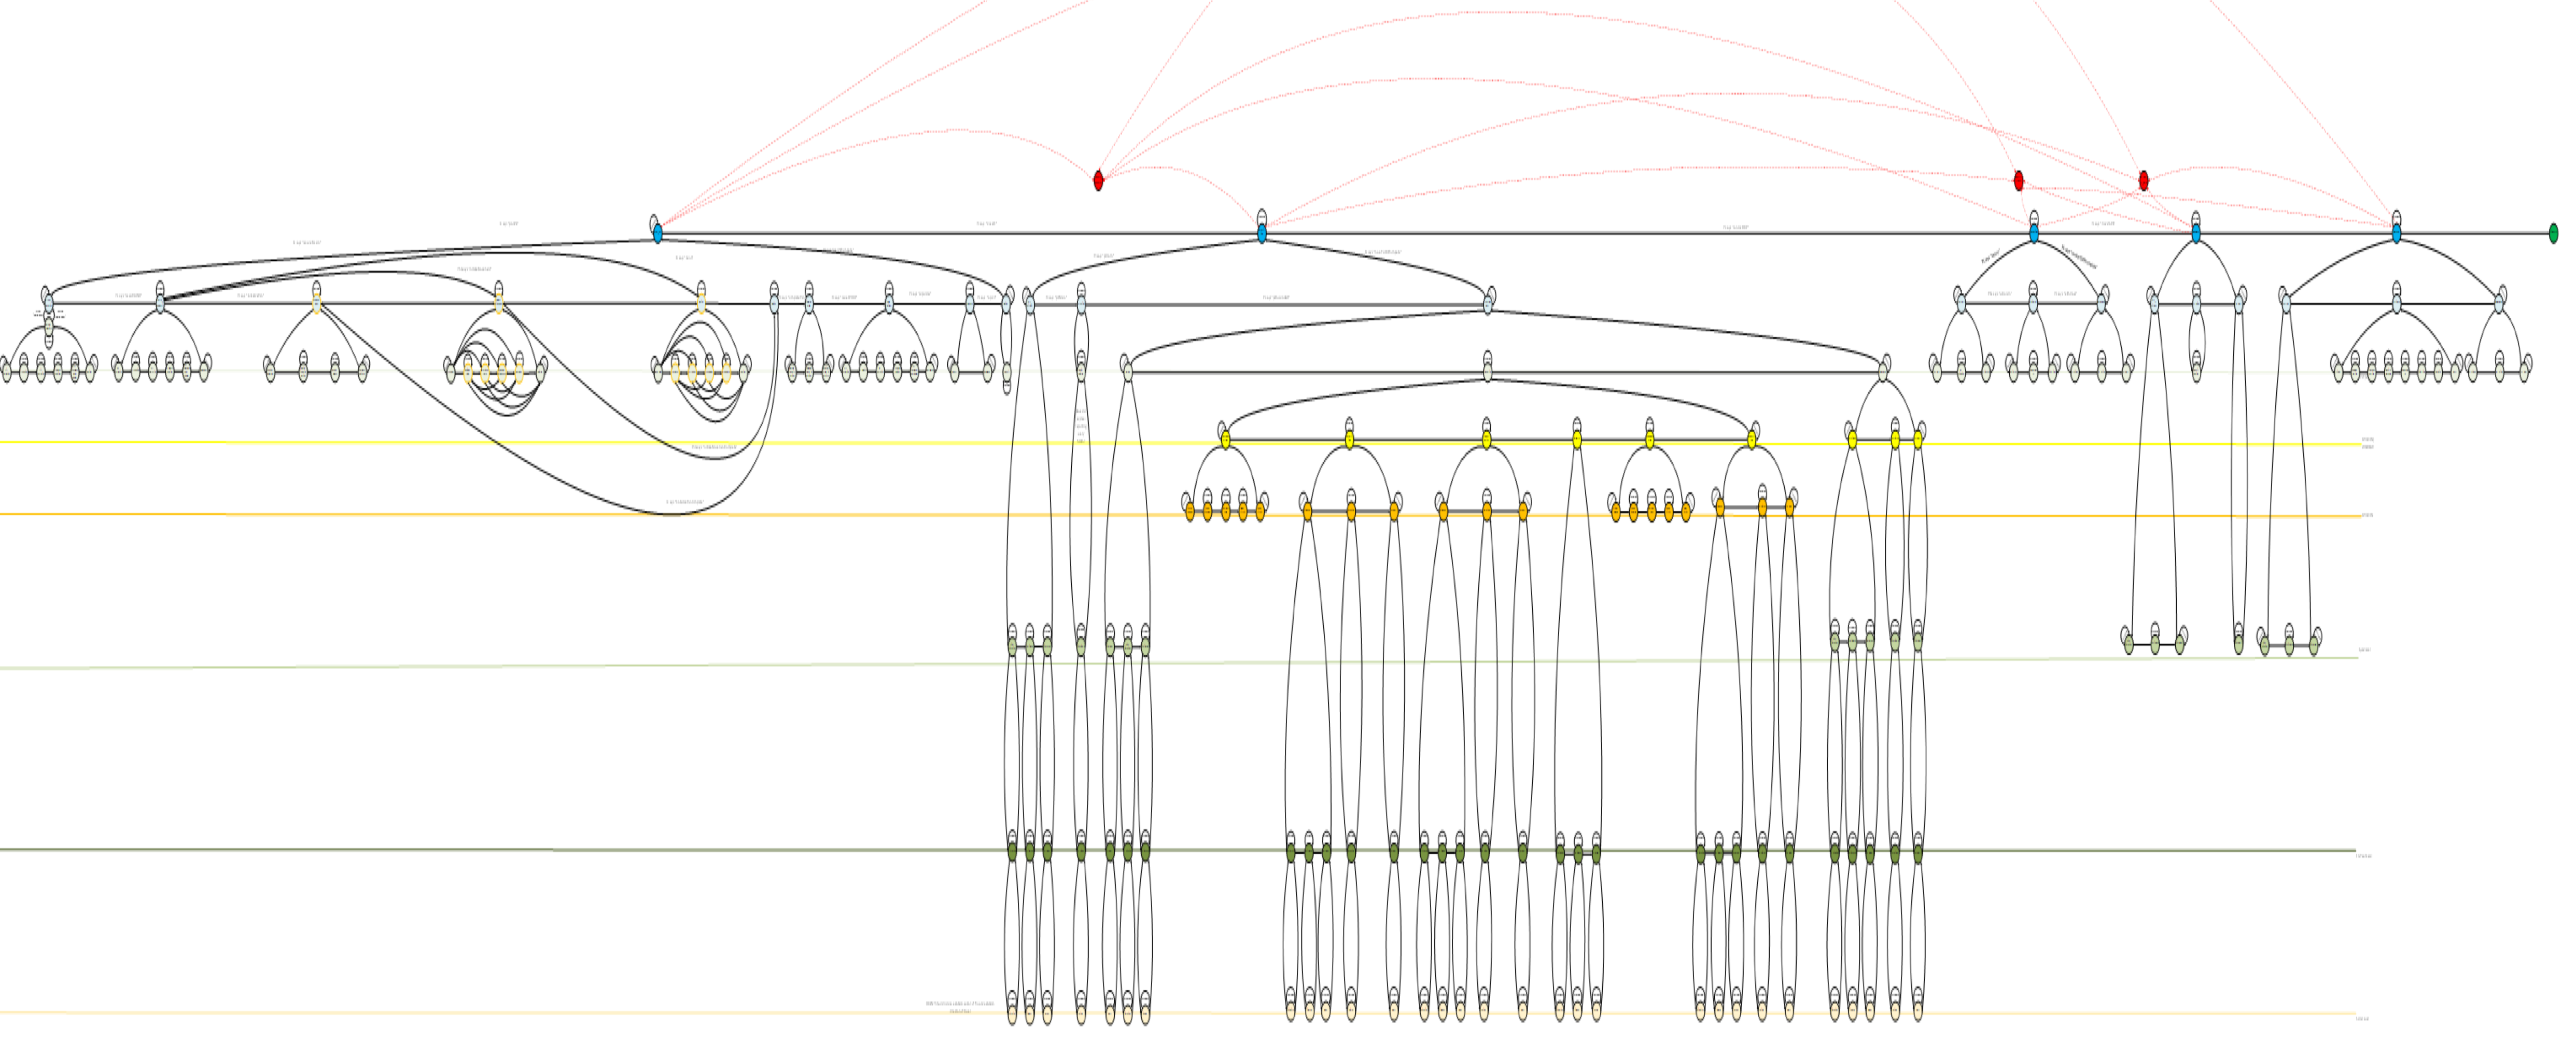
\includegraphics[width=\textwidth]{../figures/overalldiagramsquashed.png}
\caption{This is a caption for this figure.}
\end{figure}


          %%%%%%%%%%%%%%%% Subsection Diagrammatic Description %%%%%%%%%%%%%%
\subsection{Diagrammatic Description in Visio}\label{ssec:overalldiagram}
\begin{figure}[t]
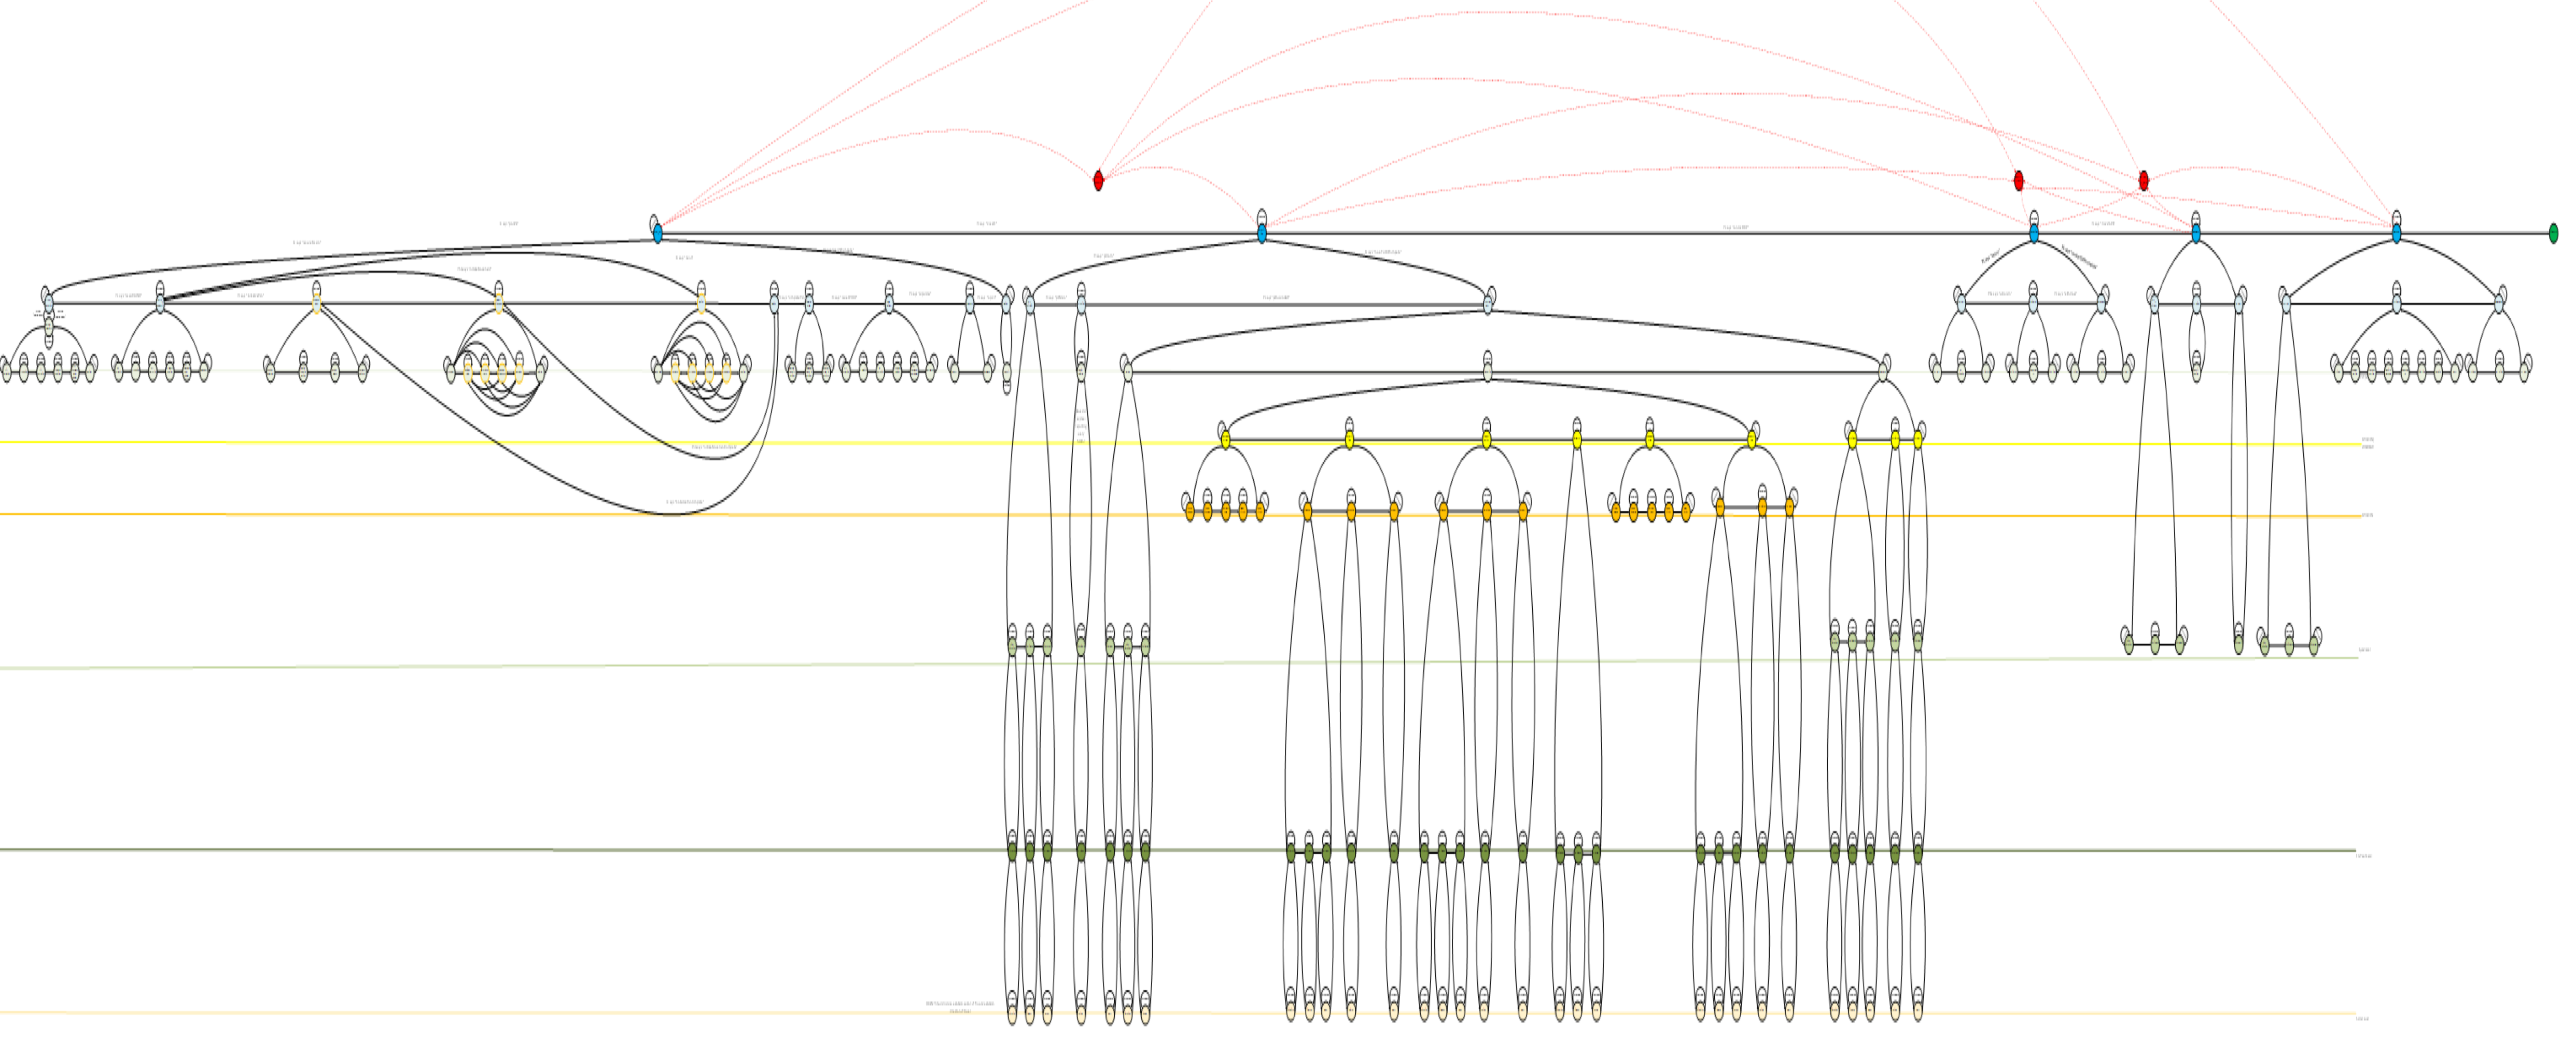
\includegraphics[width=\textwidth]{../figures/overalldiagramsquashed.png}
\caption{Diagrammatic description of patrol base operations as a hierarchy of secure state machines.  (Generated by Jesse Nathanial Hall.)}
\end{figure}

          %%%%%%%%%%%%%%%% Subsection OMNI-Level %%%%%%%%%%%%%%%%%%%%%
\subsection{OMNI-Level}\label{ssec:omnilevel}

          %%%%%%%%%%%%%%%% Subsection Escape %%%%%%%%%%%%%%%%%%%%%%%
\subsection{Escape}\label{ssec:escape}

          %%%%%%%%%%%%%%%% Subsection Top Level %%%%%%%%%%%%%%%%%%%%%%
\subsection{Top Level}\label{ssec:toplevel}

          %%%%%%%%%%%%%%%% Subsection Horizontal Slice %%%%%%%%%%%%%%%%%%%
\subsection{Horizontal Slice}\label{ssec:horizontalslice}

                  %%%%%%%%%%%%% Subsection ssmPlanPB %%%%%%%%%%%%%%%%%%%%%
\subsubsection{ssmPlanPB}\label{sssec:ssmPlanPB}

                  %%%%%%%%%%%%% Subsection ssmMoveToORP %%%%%%%%%%%%%%%%%%%
\subsubsection{ssmMoveToORP}label{sssec:ssmMoveToORP}

                  %%%%%%%%%%%%% Subsection ssmConductORP %%%%%%%%%%%%%%%%%%
\subsubsection{ssmConductORP}label{sssec:ssmConductORP}

                  %%%%%%%%%%%%% Subsection ssmMoveToPB %%%%%%%%%%%%%%%%%%%
\subsubsection{ssmMoveToPB}label{sssec:ssmMoveToPB}

                  %%%%%%%%%%%%% Subsection ssmConductPB %%%%%%%%%%%%%%%%%%%
\subsubsection{ssmConductPB}\label{sssec:ssmConductPB}

          %%%%%%%%%%%%%%%% Subsection Vertical Slice %%%%%%%%%%%%%%%%%%%%
\subsection{Vertical Slice}\label{ssec:verticalslice}

                  %%%%%%%%%%%%% Subsection ssmSecureHalt %%%%%%%%%%%%%%%%%%%
\subsubsection{ssmSecureHalt}\label{sssec:ssmSecureHalt}

                  %%%%%%%%%%%%% Subsection ssmORPRecon %%%%%%%%%%%%%%%%%%%
\subsubsection{ssmORPRecon}\label{sssec:ssmORPRecon}

                  %%%%%%%%%%%%% Subsection ssmMoveToORP4L %%%%%%%%%%%%%%%%%
\subsubsection{ssmMoveToORP4L}\label{sssec:ssmMoveToORP4L}

                  %%%%%%%%%%%%% Subsection ssmFormRT %%%%%%%%%%%%%%%%%%%%
\subsubsection{ssmFormRT}\label{sssec:ssmFormRT}


\end{document}